% This is the appendix, to be put at the end of the article, to describe pp efficiency
\label{sec:EfficiencyAppendix}
\addtocontents{toc}{\protect\setcounter{tocdepth}{0}}
\section{Photon Efficiency: p-Pb}
In this section, the $\gamma$ efficiency of the EMCal for the p-Pb is determined using the gamma-jet Monte Carlo 17g6a1. A ratio is taken according to equation~\ref{eq:eff}. The resulting ratio is the efficiency as a function of \pt for photons in the EMCAL only, as there was no DCAL duing this time period. The efficiency is rather flat and independent of \pt as seen in figure~\ref{fig:photonEff_pPb}. When applied a constant fit from 12 GeV to 40 Gev, we get an fficiency of $0.788 \pm 0.002$ with an efficiency of 0.777 at 12 GeV and at 0.785 at 40 GeV which is less than 1\% variation between the high and low of our trigger photon energy range. 
\begin{figure}
\centering
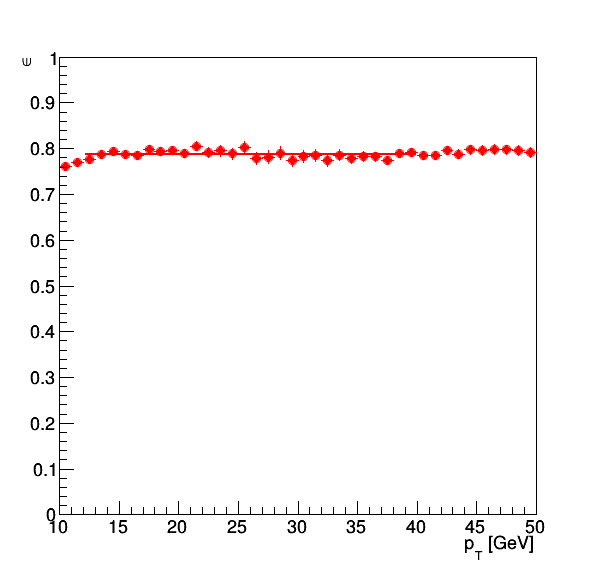
\includegraphics[width=0.7\textwidth]{EfficiencyAppendix/Efficiency_photon_pPb.png}
\caption{The photon efficiency in the EMCAL for the p-Pb Monte Carlo.}
\label{fig:photonEff_pPb}
\end{figure}

%\section{Photon Efficiency: pp}
%In this section, the $\gamma$ efficiency of the EMCal and DCal is determined using the 18b10a and 18b10b simulations. The 18b10a simulates the EMCal, while the 18b10b simulates the DCal. The cutflow for photon selection is the same as mentioned in Table~\ref{ClusterCutFlow_pp}. An additional cut is made in order reject the truth photons in the PHOS, which sits in the gap in the DCAL. Two histograms are filled. The first histogram contains the generated truth photons $\eta,\phi$ distribution, while the other contains the reconstructed truth photon $\eta, \phi$. The $\eta$ and $\phi$ distribution of the photons are shown in Figure~\ref{fig:2Dpp}. The simulation generates photon within the region of the PHOS, and so cuts of $|\eta| > 0.12$ and $-1.745 < \phi < -0.698$ have also been applied in order to reject the photons in the PHOS as they would incorrectly reduce the DCAL efficiency.

%A ratio is taken according to equation~\ref{eq:eff}. The resulting ratio is the efficiency in $\eta$ and $\phi$ for the EMCAL and the DCAL. The efficiency plots are shown in Figure~\ref{fig:AppendixEfficiencies}. The reconstruction efficiency is 0.89 for photons from the pPb dataset while 0.92 for the pp-EMCAL.
%\begin{figure}
%\centering
%\includegraphics[width=0.7\textwidth]{EfficiencyAppendix/photon_etaPhi.pdf}
%\caption{The $\eta$ and $\phi$ distributions for the generated truth photons (bottom), and reconstructed truth photons %(top).}
%\label{fig:2Dpp}
%\end{figure}

%\begin{figure}
%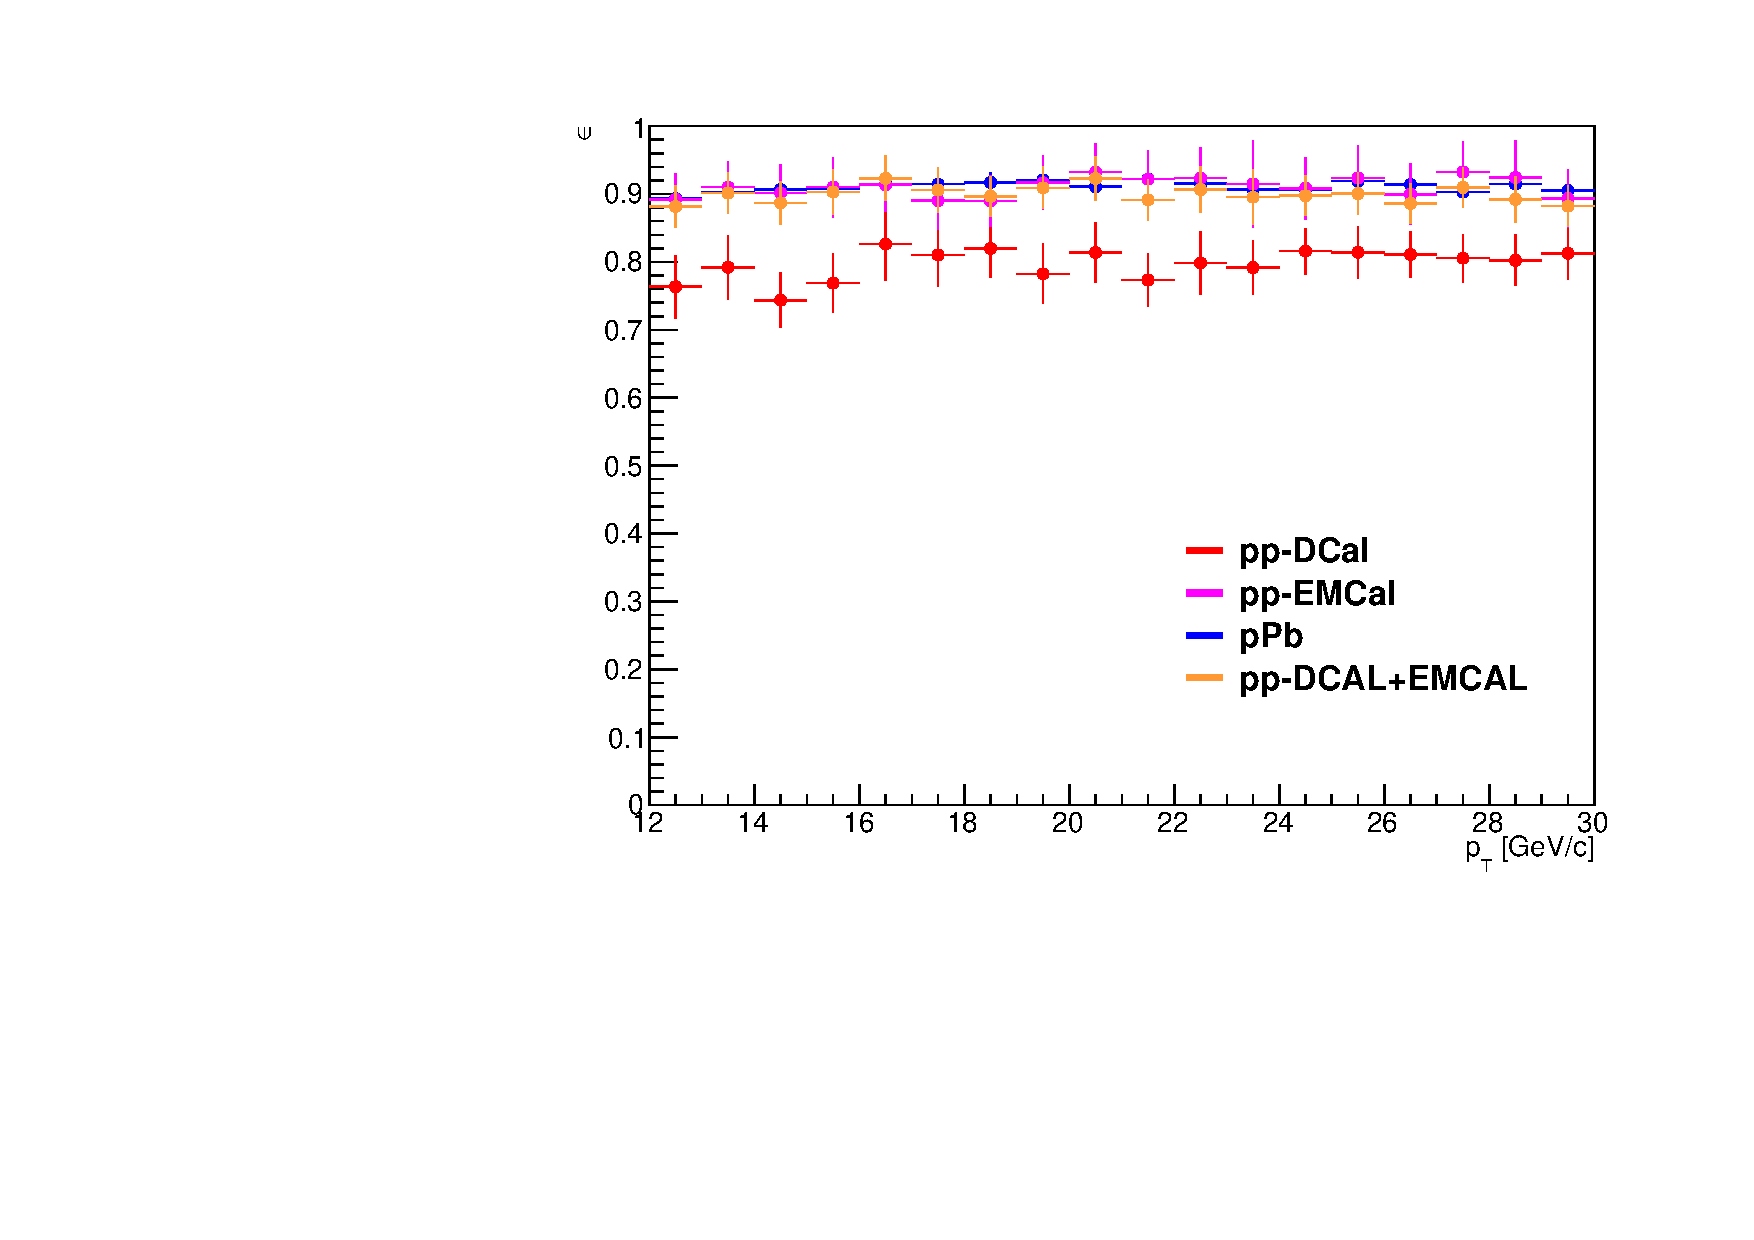
\includegraphics[width=0.5\textwidth]{EfficiencyAppendix/EfficiencyComparison_photons.pdf}
%\includegraphics[width=0.5\textwidth]{EfficiencyAppendix/photon_etaPhiEff.pdf}
%\caption{On the left, efficiency of the EMCal and DCal with respect to $p_T$. On the right, efficiency of the DCal (low $\phi$) and EMCal %(high $\phi$)}
%\label{fig:AppendixEfficiencies}
%\end{figure}
%As seen in Figure~\ref{fig:AppendixEfficiencies} the DCal tends to have a lower efficiency than the EMCal, and that is likely due to bad channels being more abundant in the DCal, as aside from the bad cells, efficiency in the $\Delta$ $\phi$-$\Delta$ $\eta$ efficiency chart is pretty uniform and it's clear that the DCal has more bad cells. \textbf{[The DCAL efficiencies are missing because of low statistics. Will be updated promptly once the analysis done over more statistics.]}


%\begin{figure}
%\centering
%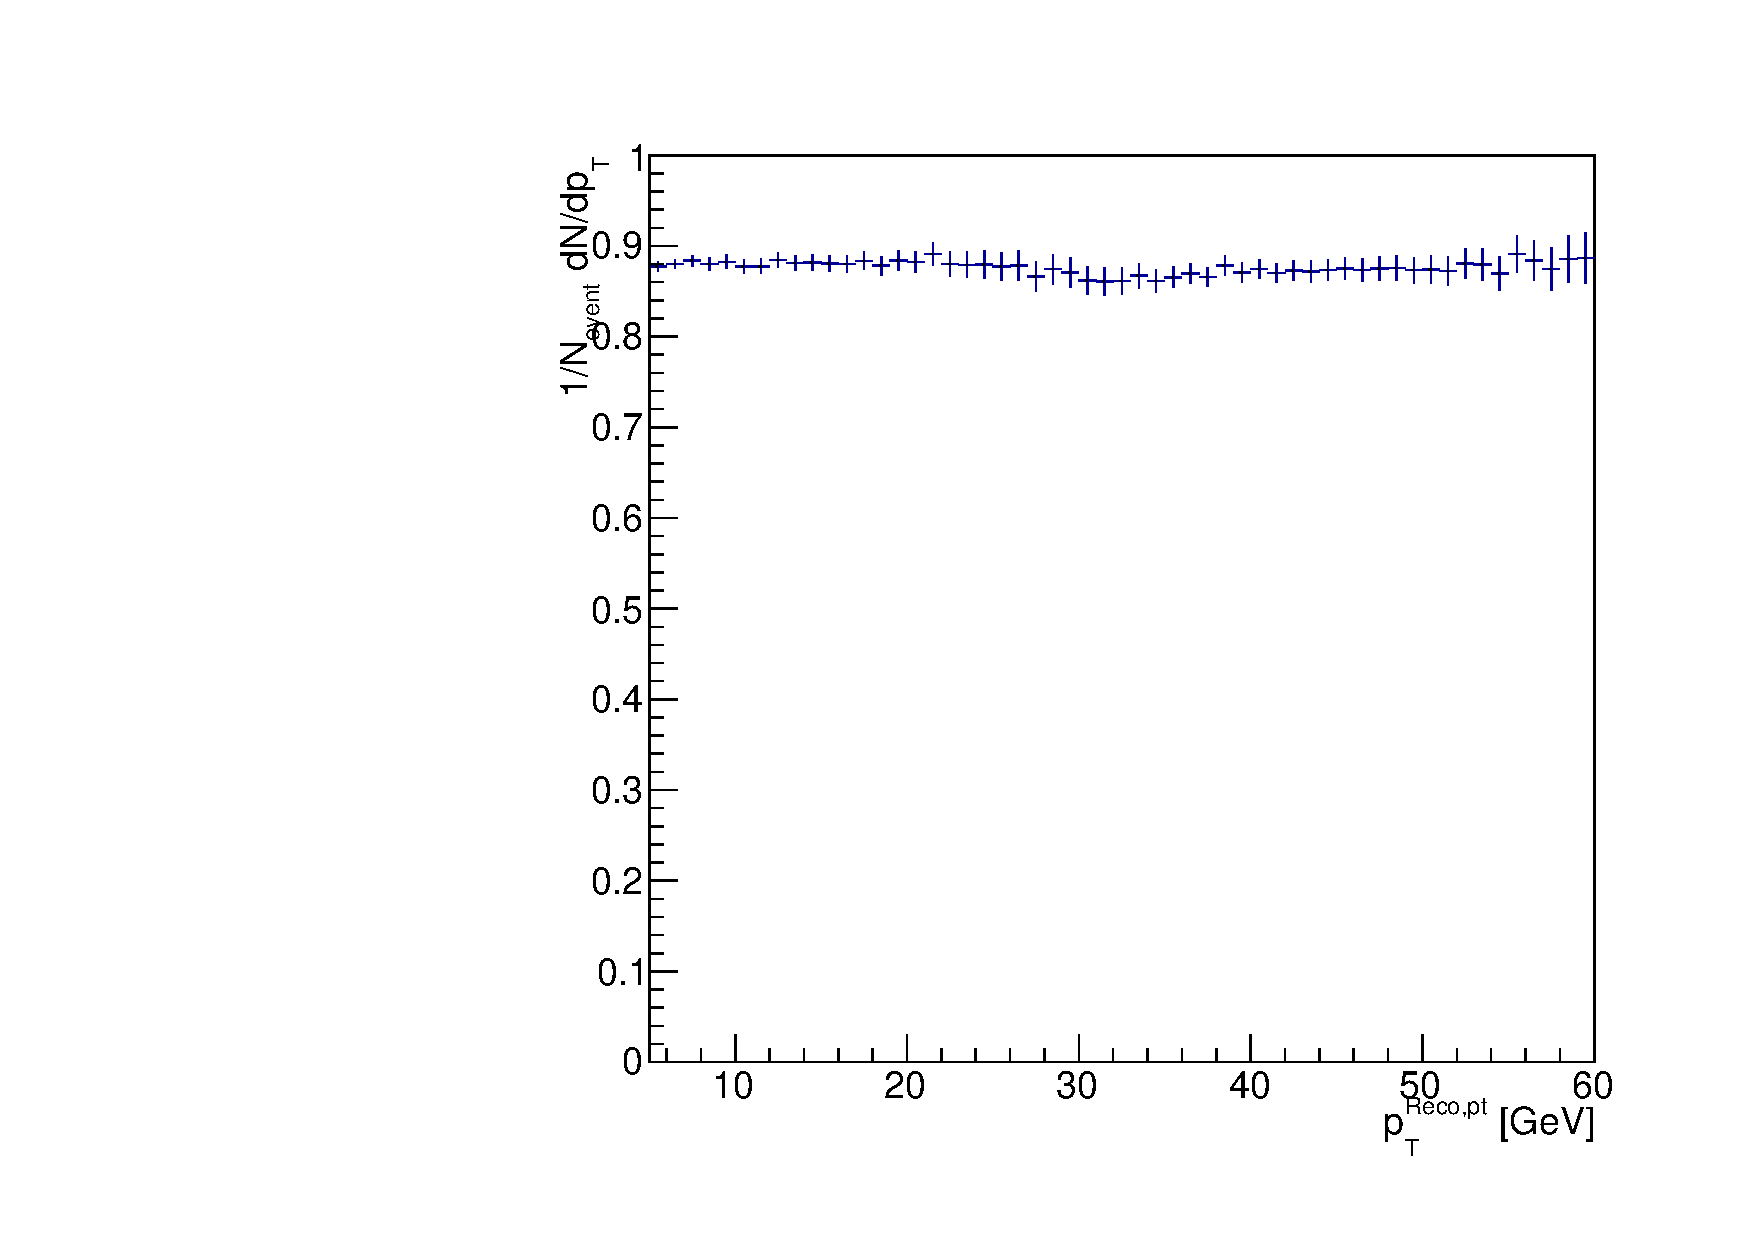
\includegraphics[width=0.7\textwidth]{EfficiencyAppendix/isoEff.pdf}
%\caption{The efficiency due to the isolation cut is calculated as the ratio of photons which pass the isolation criteria divided by all %the photons.}
%\label{fig:isoEff}
%\end{figure}

%The isolation efficiency is ratio of the numbers of photons which pass the all of the cuts mentioned in Table~\ref{ClusterCutFlow_pp} divided by the number of photons which all cuts without applying the isolation cut.
%\begin{equation}
%\epsilon(\pt^{reco}) = \frac{N^{all cuts + ISO cut}(\pt^{reco})}{N^{all cuts}(\pt^{reco})}
%\end{equation}
%The isolation efficiency is calculated to be 0.88 by applying a constant fit to the ratio shown in Figure~\ref{fig:isoEff}.





